\documentclass[10pt]{article}
\usepackage{latexsym}
\usepackage{natbib}
\usepackage{graphicx}
\usepackage{subfigure}
\usepackage{listings}
\usepackage{algorithm}
\usepackage{algpseudocode}

\title{Homework 1: Eigendigits}
\author{Shun Zhang}
\date{}

\begin{document}
\maketitle

\section{Introduction}

In this report, I applied principal components analysis on digits
classification problem.

In our example, the original figures are represented in
728-dimensional vectors. This is a comparatively high dimensional
representation. Distance of vectors in this space would be very large.
This fact is also known as ``curse of dimension''. It would be low
efficient to do learning in this high-dimensional space, so reduction
on dimension is necessary.

However, figures of digits should be easy to describe - they need far
less than 728 dimensions. The motivation is that we want use a basis
such that coordinates of the figures vary the most. This would be the
most expressive way in a limited dimension. We could look into the
covariance matrix of the data, and use its eigenvectors with maximum
eigenvalues.

\section{Algorithm}

Let a figure be in size of $n \times n$. Let $X$ be the matrix such
that each column of it is a datum, represented as an unrolled vector
of size of $n^2 \times 1$. Let there be $K$ samples. Then the
dimension of $X$ is $n^2 \times K$. The covariance of $X$ is defined
as,
$$Cov(X) = \mathrm{E}((X - \mathrm{E}(X))(X - \mathrm{E}(X))^T)$$
Let $A = X - \mathrm{E}(X)$. As $A$ is in $n^2 \times n^2$ dimension,
we don't want to find eigenspace for this directly. As we know,
$$A^TAx = \lambda x$$
$$AA^TAx = \lambda Ax$$
we can find eigenvectors of $A^TA$, and lefty multiply them with $A$
to get eigenvectors of $AA^T$.

\begin{figure}
\centering
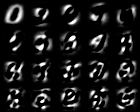
\includegraphics[]{eigen.png}
\caption{First 20 eigenvectors, using first 2000 training samples.
They are aligned from left to right and then top to down. They become dark
after normalization. So in this figure, each value is multiplied by
10, i.e., each vector has norm of 100, instead of 1. }
\label{fig:eigen}
\end{figure}

Let $V$ be the set of the eigenvectors of $AA^T$, sorted descending
according to the eigenvalues. It's actually a set of basis we want to
use. The first 20 eigenvectors are shown in Figure~\ref{fig:eigen}.
Intuitively, eigenvectors with smaller eigenvalues care more about
details of the digits, while the ones with higher eigenvalues care
more about predominant features of the digits.

If we call the basis we use as $B$ and the eigenspace as $E$. $V$
is a linear transformation from $E$ to $B$, usually represented as
$P_{BE}$ in the linear algebra literature. We also need $P_{EB}$,
which is defined as the inverse of $P_{BE}$. We know that $P_{BE}$ is
orthogonal, because it's the covariance matrix of a symmetric matrix.
Therefore, $P_{EB} = P_{BE}^T$.

Now, we can transform any vector in $B$ or $E$ basis to the other in
the following way.
$$[v]_E = P_{EB} [v]_B$$, which maps a vector from original space to
the eigenspace.
$$[v]_B = P_{BE} [v]_E$$, which maps a vector from the eigenspace to
the original space.

\begin{figure}
\centering
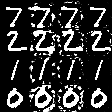
\includegraphics[]{test.png}
\caption{Reconstruction of digits. From left to right on each line,
there are original digits, digits constructed by first 100
eigenvectors, digits constructed by first 200 eigenvectors, and digits
constructed by first 600 eigenvectors. }
\label{fig:test}
\end{figure}

We can check how digits are ``reconstructed'' after mapping from $B$ to
$E$ and then back to $B$. Figure~\ref{fig:test} shows the
reconstruction result, using 100, 200, and 600 eigenvectors
respectively. The more eigenvectors used, the more close it
reconstructed, and, as a cost, the higher the dimension of $E$ is.

In the following part of this section, I describe two algorithms I
used for classification.

\subsection{K-Nearest-Neighbors}

This is the algorithm that making the neighbors of a given data point
to determine its label. I transform the training set from $B$ to $E$ to
reduce its dimension. For a test sample, say $u$, I also transformed
it to $E$ space, as $[v]_E$. I compute the distance of this to every
training sample. The k training samples with smallest distance are
selected. They majority of their labels is considered as the label of
this test datum.

\subsection{Maximum Likelihood Estimation}

Different from K-Nearest-Neighbors, this assumes Gaussian-like
distribution of each class. Assume the prior distribution for each class
is uniform. Mean and variance for data in each class
are computed. Then we can compute the posterior probability of a datum
given each class. We determine the label by picking the class with
largest probability to own this datum.

\section{Experiments}

%hw1Classify(n, 1000, 200, 1)
\begin{figure}
\centering
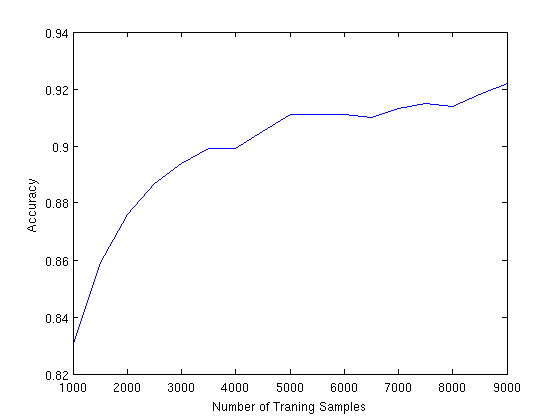
\includegraphics[width=0.55\columnwidth]{diffDataSet.png}
\caption{Comparison on using different number of training samples on
different types of classification algorithms, indicated in the legends.
Testing on first 1000 testing set. Using first 50 eigenvectors.}
\label{fig:dataset}
\end{figure}

Figure~\ref{fig:dataset} shows result of the learning performance on
different size of data, using different type of classification
algorithms. Overall, it's not surprising that the more training data
provided, the better accuracy can be achieved.

The maximum likelihood estimation has the best performance. It takes
the mean and variance of all the classes into consideration. In
contrast, KNN would have difficulty in identifying data on the
"boundary" between classes, or when two classes are not fully
disjunct. In the latter case, mean and variance of two classes can
describe the distribution well, while KNN, which only looks into the
local points near the test datum, would be less likely to identify its
class.

Apart from this, the distribution pattern of a class can also
harm the performance of KNN\@. Suppose a class has a narrow but long
distribution, then KNN would count the surrounding data from other
classes. Because of cases like this, we can observe that $K=30$ has a
worse performance than $K=5$.

\hfill

\begin{figure}
\centering
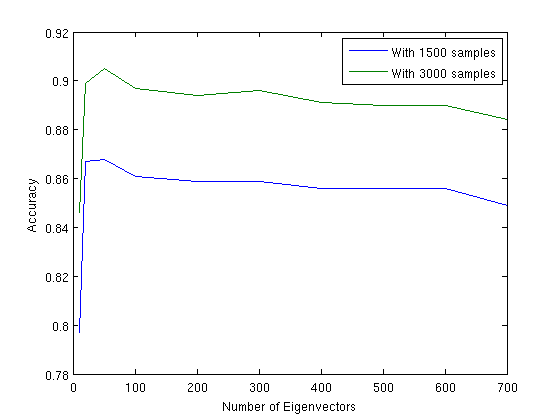
\includegraphics[width=0.55\columnwidth]{diffEVector.png}
\caption{Comparison on using different number of eigenvectors.
Testing on first 1000 testing set. Using first 1500 and 3000 training
samples for each line.  K for K-Nearest-Neighbors is 1.}
\label{fig:evec}
\end{figure}

Figure~\ref{fig:evec} shows the learning performance on different set
of eigenvectors. I used Nearest-Neighbor algorithm ($K = 1$ for KNN),
as this is the most naive way to do classification, and what I want to
compare in this experiment is the number of eigenvectors.

Here is some interesting observation. When too few
eigenvectors are used, which means $E$ has very small dimensions, the
accuracy is low. This is because vectors in $E$ are not expressive
enough. However, when there are too many eigenvectors provided, the
learning performance would go worse, as it's hard to learn in a high
dimensional space.  Figure~\ref{fig:evec} shows that 50-100
eigenvectors have the best performance, when the training set is
fixed.

\hfill

\begin{figure}
\centering
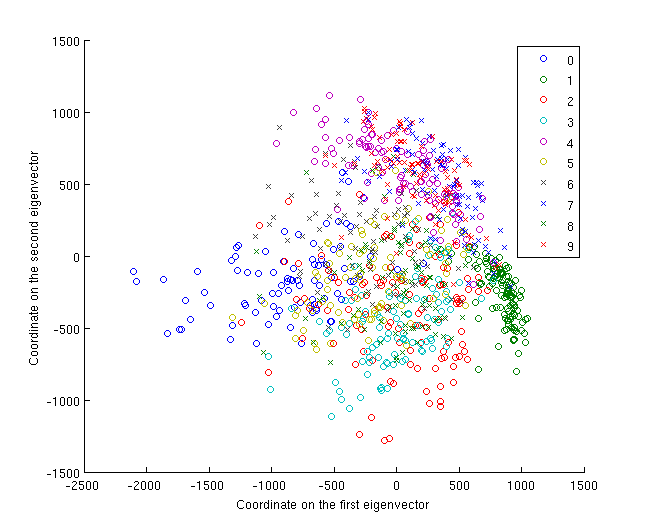
\includegraphics[width=0.55\columnwidth]{twod_digit.png}
\caption{Data coordinates on first two basis in $E$ space.  Using
first 5000 training samples. Testing on first 1000 testing samples.}
\label{fig:twod}
\end{figure}

\begin{figure}
\centering
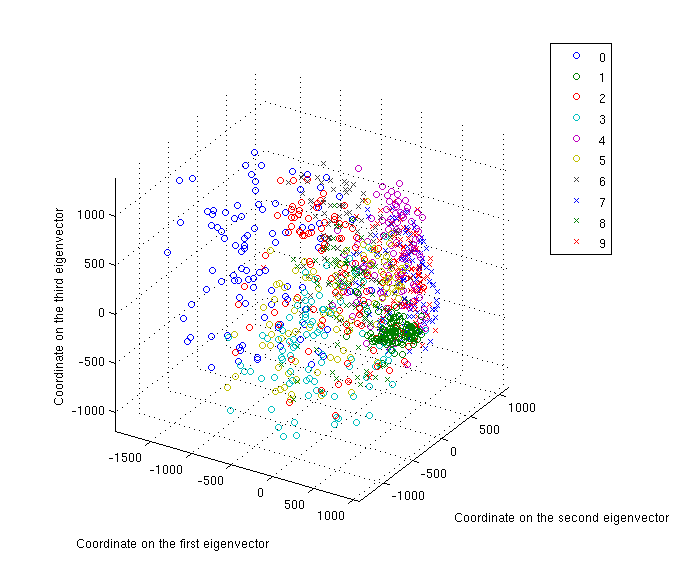
\includegraphics[width=0.55\columnwidth]{threed_digit.png}
\caption{Data coordinates on first three basis in $E$ space.  Using
first 5000 training samples. Testing on first 1000 testing samples.}
\label{fig:threed}
\end{figure}

Another interesting thing to check is to show the distribution of data
in the eigenspace. I draw the coordinates of different
set of digits in $E$. Figure~\ref{fig:twod} shows the coordinates of
data in $E$ basis, but only on first two eigenvectors.
Figure~\ref{fig:threed} shows them on first three eigenvectors (it's
worth looking at it, even it's hard to read data from a 3 dimensional
space). They
spread the most on the first basis, which is the x axis, and less, but
still much, on the second basis, which is the y axis, and even less on
the z axis.

They have some clustering performance, while not disjunct. They also
have different patterns - for example, $0$ has a wide distribution,
while $1$ has a narrow but long distribution. This is because we
didn't take labels into consideration when designing the $E$ basis.
$E$ basis makes data representation more efficient, but doesn't help
to separate data from different labels. The performance of clustering
in the figure is caused by the nature of difference looking of
figures.

\section{Conclusion}

In this assignment, I implemented principal components analysis to
classify digits in the eigenspace of the covariance matrix of the
data. This reduces the dimension of the data, with the least
information loss. Therefore, this can be generally used for
compressing data into lower dimension.

I found that maximum likelihood estimation has the best performance on
classification on digits. This is because it considers the
distribution of each classes, and the data from different classes have
Gaussian distributions.

However, by observing the result in Figure~\ref{fig:twod}, I believe
that $E$ could be more carefully selected, which makes data in
different classes more separable for classification purpose.

\end{document}
